\section{Metodologia}
\label{sec:methodology}

Este capítulo apresenta a metodologia para avaliar como perturbações ambientais 
e climáticas reduzem a acessibilidade urbana e afetam diferentes grupos sociais. 
O método consiste em comparar quantitativamente dois cenários da rede de deslocamento: 
um com condições típicas e outro modificado por variáveis ambientais. Essa 
comparação permite isolar, quantificar e mapear as perdas de acesso às oportunidades 
na cidade.

O fluxo de trabalho estrutura-se em quatro etapas principais:

\begin{enumerate}
   \item \textbf{Modelagem Territorial} (Seção \ref{subsec:territorial_modelling}): 
   Representação do espaço urbano como um sistema discreto composto por malha de 
   análise, rede viária (grafo), pontos de interesse e dados socioeconômicos;
   
   \item \textbf{Cenários e Perturbações} (Seção \ref{subsec:scenarios}): 
   Definição dos dois cenários (topologia típica vs topologia condicionada). 
   Inclui a aplicação da função de penalização ambiental nos custos da rede 
   — dinâmica central ilustrada na Figura \ref{fig:framework} — e o 
   cálculo dos indicadores de acessibilidade (PTh, Índice G e F15, conforme 
   definidos na Seção \ref{subsubsec:indicadores}) para ambos os estados;

   \item \textbf{Análise Comparativa} (Seção \ref{subsec:comparative}): 
   Quantificação das perdas de acessibilidade, mapeamento dos padrões espaciais 
   de impacto e testes de significância;
   
   \item \textbf{Análise de Desigualdade Socioeconômica} (Seção \ref{subsec:socioeconomical}): 
   Cruzamento das perdas de acessibilidade com dados de renda, escolaridade e 
   densidade populacional para identificar quais grupos e territórios são mais 
   vulneráveis.
\end{enumerate}

\begin{figure}[H]
  \centering
  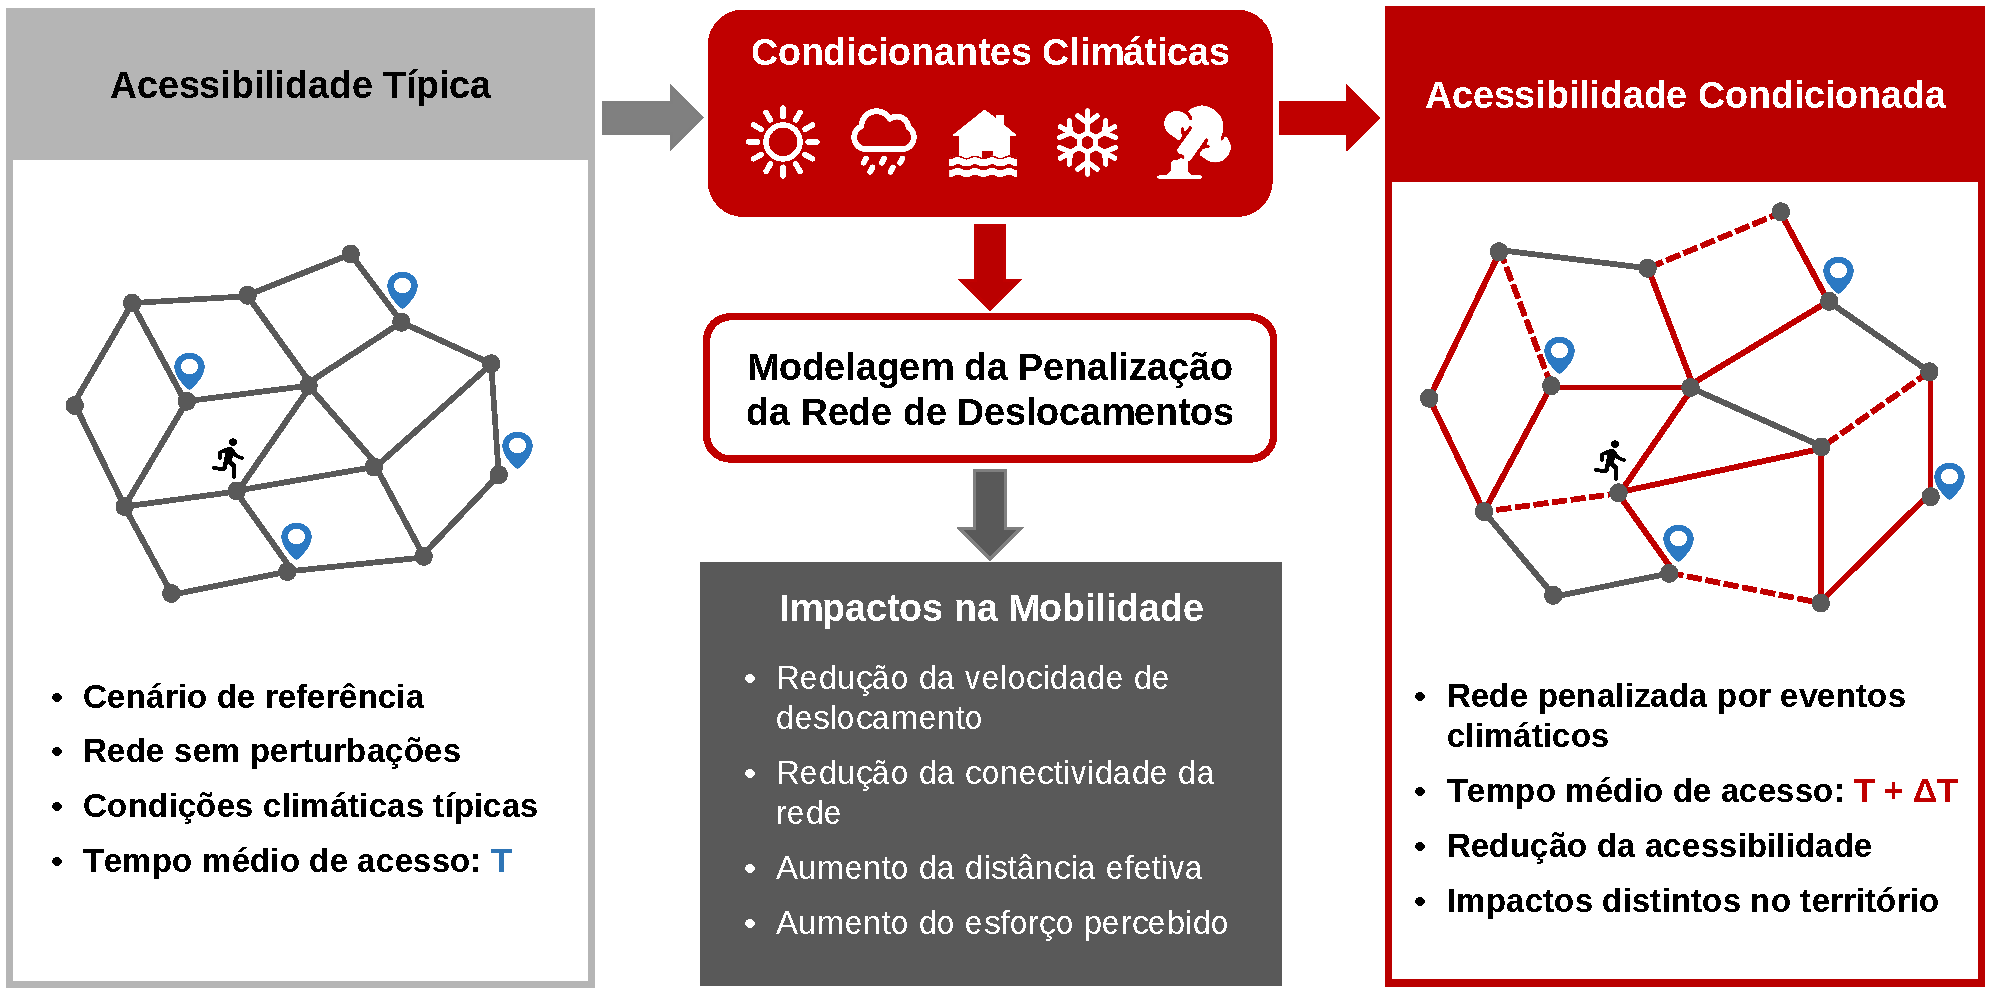
\includegraphics[width=1\textwidth]{figs/framework.pdf}
  \caption{Fluxo de modelagem dos cenários de acessibilidade. À esquerda, a rede no cenário típico, com seus custos originais de deslocamento. Ao centro, o mecanismo de penalização, que utiliza dados ambientais para penalizar a infraestrutura de mobilidade. À direita, o cenário condicionado, no qual o aumento do comprimento das arestas representa visualmente o acréscimo no tempo ou custo de deslocamento provocado pela perturbação.}
  \label{fig:framework}
\end{figure}

% O restante da Seção está estruturado da seguinte forma: a Subseção \ref{subsec:composition} apresenta o processo de coleta, pré-processamento e integração dos dados utilizados na modelagem do território urbano; a Subseção \ref{subsec:processing} descreve o método de cálculo dos indicadores de mobilidade e acessibilidade em diferentes cenários; a Subseção \ref{subsec:comparative} detalha os procedimentos para comparação entre os cenários ideal, típico e condicionado; a Subseção \ref{subsec:socioeconomical} expõe a integração de dados socioeconômicos, permitindo análises de desigualdades de acessibilidade; e, por fim, a Subseção \ref{subsec:case} explica os dados e ferramentas que serão utilizados no estudo de caso para aplicação da metodologia.

\subsection{Modelagem Territorial}
\label{subsec:territorial_modelling}

A modelagem do território urbano consiste na coleta, pré-processamento e integração de cinco camadas de dados espaciais que servem de base para a análise da acessibilidade:

\paragraph{1. Malha de análise:} Uma grade espacial regular que define a unidade mínima de estudo. A resolução da malha é ajustada ao modo de transporte e ao contexto local. O centroide de cada célula funciona como a origem teórica dos deslocamentos, servindo de base para o cálculo e a agregação dos indicadores.

\paragraph{2. Pontos de Interesse (POIs):} Representam os destinos dos deslocamentos. São coordenadas que indicam a localização dos serviços cotidianos da população, organizados em categorias (como saúde, educação e transporte). A seleção depende da disponibilidade de bases de dados locais, sejam oficiais ou colaborativas (crowdsourced).

\paragraph{3. Rede viária:} A infraestrutura de mobilidade é estruturada como um grafo espacial. Os vértices representam os cruzamentos e as arestas representam os segmentos de via, cujo peso base inicial corresponde à distância percorrida. Para possibilitar o cálculo de rotas reais, o centroide de cada célula da malha de análise é vinculado ao vértice mais próximo da rede.

\paragraph{4. Condicionantes ambientais:} Camadas espaciais, que podem ser contínuas (como imagens \textit{raster}) ou discretas (polígonos vetoriais), mapeando os fenômenos climáticos ou ambientais avaliados. Esses dados são sobrepostos à rede viária para reajustar o custo de deslocamento das arestas afetadas no cenário perturbado.

\paragraph{5. Dados Demográficos e Socioeconômicos:} Informações que caracterizam a população residente, como densidade demográfica, renda e escolaridade, oriundas de censos oficiais. Como esses dados são disponibilizados em unidades administrativas irregulares (como setores censitários), aplica-se um procedimento de compatibilização espacial para transferir o perfil socioeconômico para as células da malha regular de análise.

\subsection{Cenários e Perturbações}
\label{subsec:scenarios}

Nesta etapa, a rede de deslocamentos é avaliada em dois estados distintos: (1) Cenário Típico, que reflete as condições normais de mobilidade; e (2) Cenário Condicionado, no qual os custos da rede são alterados por variáveis ambientais.

No \textbf{Cenário Típico}, o peso de cada aresta do grafo ($W_{base}$) corresponde estritamente ao comprimento real do trecho da via. O tempo de percurso em condições normais é obtido dividindo-se essa distância pela velocidade média de deslocamento definida para o modo de transporte analisado.

No \textbf{Cenário Condicionado}, os custos de deslocamento são recalculados por meio de uma função de penalização. Esta função cruza a malha viária com as camadas de condicionantes ambientais ($C$), gerando um peso penalizado ($W_{condicionado}$) para cada aresta, estruturado na forma $W_{condicionado} = f(W_{base}, C)$. A aplicação geométrica dessa função varia conforme a natureza do dado ambiental:

\begin{itemize}
    \item \textbf{Dados contínuos} (ex.: \textit{rasters} de temperatura): O algoritmo extrai a média dos valores dos pixels que se sobrepõem geograficamente à aresta. Esse valor atua como um penalizador contínuo, aumentando o tempo de percurso proporcionalmente à severidade da condição ambiental ao longo daquele trecho.
    
    \item \textbf{Dados discretos} (ex.: polígonos de alagamento ou barreiras físicas): O algoritmo utiliza operações de interseção vetorial. A função pode aplicar multiplicadores severos ou atribuir peso infinito aos trechos interceptados, simulando interdições totais que forçam o roteamento a buscar caminhos alternativos. Essa mesma lógica de interseção pode ser usada de forma inversa, reduzindo pesos para simular áreas favoráveis (como vias arborizadas).
\end{itemize}

A forma matemática da função de penalização $f$ (linear, exponencial, limiar de corte) é um parâmetro ajustável. A escolha e calibração desses parâmetros devem considerar dados ou estudos do contexto local, já que a influência de variáveis ambientais sobre a velocidade e o esforço para caminhar varia conforme o clima, a cultura e as características urbanas. Evidências recentes mostram que fatores como temperatura, clima e condições viárias alteram significativamente o padrão e a velocidade da caminhada \cite{LIANG2020106811,Obuchi2021}. Por isso, recomenda-se que o aplicador utilize valores observados localmente ou reportados na literatura para definir as funções de penalização e os parâmetros do modelo.

Por fim, com os grafos dos dois cenários estruturados, um algoritmo de caminho de menor custo é executado para calcular as matrizes de tempo de viagem. A partir desses tempos, computam-se os indicadores apresentados na Seção \ref{subsubsec:indicadores}: o PTh de cada unidade territorial, o índice G (desigualdade) e o F15 (fração da população atendida) para ambos os cenários.

\subsection{Análise Comparativa}
\label{subsec:comparative}

Nesta etapa, quantificam-se as perdas de acessibilidade comparando diretamente os indicadores do cenário típico com os do cenário condicionado. O objetivo é mensurar a degradação da mobilidade imposta pelos fatores ambientais e identificar pontos críticos onde a dificuldade de circulação provoca maior isolamento.

Essa comparação é estruturada em três procedimentos analíticos principais:

\begin{itemize}
    \item \textbf{Variação relativa:} Cálculo das diferenças absolutas e percentuais dos tempos de deslocamento e dos níveis de acesso entre os dois cenários, evidenciando a magnitude da perda para cada unidade da malha.
    \item \textbf{Validação estatística:} Aplicação de testes de hipótese para confirmar a significância das alterações nos tempos de acesso provocadas pela perturbação ambiental em relação à rede original.
    \item \textbf{Mapeamento espacial:} Uso de métodos de associação local ou clusterização sobre as diferenças de tempo. Isso permite identificar, agrupar e mapear as manchas de degradação, revelando geograficamente as áreas mais penalizadas da cidade.
\end{itemize}

\subsection{Análise de Desigualdade Socioeconômica}
\label{subsec:socioeconomical}

Nesta etapa, as perdas de acessibilidade são analisadas em conjunto com os atributos socioeconômicos da população, com o objetivo de identificar padrões de vulnerabilidade associados às perturbações ambientais.

Cada célula da malha de análise, já associada aos dados sociodemográficos por compatibilização espacial, é tratada como unidade de observação. Para cada célula, consideram-se tanto os indicadores de acessibilidade no cenário típico ($PT_h$) quanto as variações induzidas pela perturbação ($\Delta PT_h$).

Inicialmente, aplica-se um modelo de regressão linear, no qual $PT_h$ e $\Delta PT_h$ são utilizados como variáveis dependentes em especificações distintas. As variáveis independentes incluem renda média, nível de escolaridade, densidade populacional e demais indicadores disponíveis. Esse procedimento permite estimar a associação entre características socioeconômicas e níveis de acessibilidade, bem como sua variação sob condições adversas.

Complementarmente, realiza-se uma análise de agrupamento socio-espacial, na qual as células são agrupadas considerando simultaneamente sua proximidade geográfica e a similaridade em termos de atributos socioeconômicos e indicadores de acessibilidade. Esse procedimento resulta em regiões adjacentes e internamente homogêneas, permitindo identificar padrões territoriais de desigualdade e vulnerabilidade de forma integrada.

% https://geoportal.sgb.gov.br/geosgb/
\subsection{Estudo de Caso}
\label{subsec:case_study}

Para demonstrar a viabilidade da metodologia proposta, o modelo será aplicado em duas capitais brasileiras: Curitiba (PR) e Porto Alegre (RS). A escolha desses municípios permite testar os dois comportamentos da função de penalização definidos na Seção \ref{subsec:scenarios}: o impacto de perturbações ambientais contínuas (temperatura de superfície) e discretas (áreas de risco geológico).

Para garantir a reprodutibilidade da pesquisa, os experimentos priorizam a utilização de dados abertos e bases governamentais oficiais.

\subsubsection{Curitiba: Degradação por Variável Contínua (Clima)}
O experimento em Curitiba avaliará como o desconforto térmico afeta a mobilidade ativa. Neste cenário, a temperatura de superfície atuará como um penalizador contínuo do esforço de deslocamento, aumentando o peso das arestas mais expostas ao calor. Os dados utilizados compreendem:

\begin{itemize}
    \item \textbf{Malha de deslocamento:} Rede viária extraída do OpenStreetMap (OSM), filtrada para infraestrutura caminhável.
    \item \textbf{Pontos de Interesse (POIs):} Coletados via OSM, complementados e validados por bases de alvarás municipais da Prefeitura de Curitiba, categorizados por tipos de serviço.
    \item \textbf{Condicionante ambiental:} Imagens de satélite (\textit{rasters}) do produto \textit{Surface Temperature} obtidas via Earth Explorer (Landsat 8 e 9, sensor TIRS - banda ST\_TRAD).
\end{itemize}

\subsubsection{Porto Alegre: Degradação por Variável Discreta (Risco Físico)}
O experimento em Porto Alegre analisará o impacto de áreas de risco geotécnico e físico sobre a acessibilidade urbana. Como condicionantes ambientais, serão utilizadas camadas vetoriais (polígonos) de \textit{Áreas com Risco a Movimentos de Massa} e \textit{Áreas de Risco Geológico}, ambas disponíveis no portal GeoPOA\footnote{\url{https://gis-smamus.portoalegre.rs.gov.br/dmweb-2-0/}} e resultantes de mapeamento realizado pelo Serviço Geológico do Brasil (SCG/CPRM). Essas áreas atuam como variáveis discretas, simulando barreiras que interrompem ou penalizam rotas afetadas por riscos. Os dados considerados para o experimento são:

\begin{itemize}
    \item \textbf{Malha de deslocamento:} Rede viária extraída do OpenStreetMap (OSM);
    \item \textbf{Pontos de Interesse (POIs):} Serviços e instalações mapeados integralmente a partir do OSM;
    \item \textbf{Condicionantes ambientais:} Polígonos das \textit{Áreas com Risco a Movimentos de Massa} e \textit{Áreas de Risco Geológico} proveniente do GeoPOA (origem: SCG/CPRM).
\end{itemize}

Por fim, para a análise de desigualdade socioeconômica em ambos os municípios, as malhas territoriais serão enriquecidas com dados do Censo Demográfico do IBGE (Instituto Brasileiro de Geografia e Estatística), permitindo o cruzamento das perdas de acessibilidade com variáveis de renda, infraestrutura domiciliar e vulnerabilidade social.

\subsection{Limitações}
\label{subsec:limitations}

A calibração dos efeitos ambientais no modelo é limitada pela disponibilidade e qualidade dos dados ou por falta de estudos específicos. Por isso, os valores de indicadores como o PTh podem não representar tempos absolutos reais, sendo mais adequados para análises comparativas entre diferentes regiões do que para estimativas precisas de tempo. Dessa forma, o modelo cumpre melhor o papel de identificar padrões de desigualdade e vulnerabilidade territorial diante de perturbações ambientais do que de quantificar o tempo exato de acesso.

Além disso, há limitações relacionadas ao comportamento dos indivíduos. Em situações extremas, as pessoas podem optar por não se deslocar ou escolher modos de transporte diferentes da mobilidade ativa. O modelo pressupõe a manutenção do deslocamento a pé mesmo sob condições adversas, o que pode não refletir a realidade observada. Assim, os resultados simulam apenas o impacto potencial das perturbações na acessibilidade da rede, não substituindo análises que considerem efetivamente as escolhas modais dos usuários. Ressalta-se, ainda, que a metodologia pode ser adaptada para outros modos de transporte, mediante ajustes nos parâmetros de velocidade e custo.

Ainda, os indicadores calculados refletem apenas o potencial de acesso espacial e o esforço exigido para atingir determinados destinos, sem considerar fatores como a qualidade, capacidade, funcionamento ou atratividade dos serviços presentes nos POIs. Além disso, esses indicadores não capturam obstáculos subjetivos, como percepção de segurança, conforto ou preferência individual de rotas. Por isso, apesar de úteis para análise territorial comparativa, os resultados não devem ser interpretados como medida direta da experiência do usuário ou garantia de acesso efetivo aos serviços analisados.






